
\documentclass{uonmathreport}

% this allows one to include .jpg etc figures using pdflatex
% change the optional argument if you use dvips or others
\usepackage[pdftex]{graphicx}


% other packages that maybe of use include:
% hyperref, amsthm, xy, todonotes, showkeys, ...

% change to \PJS or \DIS or \HGDIS (for BSc and MPhil)
% or \MSc (for all Msc dissertations)
\MSc

% adjust the following
\title{An Adaptive Finite Element Method Approach to the Heat Equation and the Black-Scholes Equation}
\author{Thabo Miles 'Matli}
\academicyear{2017/2018}
\supervisor{Dr. Kris Van Der Zee}

% the following are irrelevant for Msc:
\assessmenttype{Review} % or Investigation
\projectcode{XX P99}

% the following are irrelevant for PJS, PJA, DIS and HG4DIS:
% Msc: change it to G1PMD and Pure Mathematics, etc ...
\msccode{G14SCD}
\msctitle{Scientific Computation}

% gives double-spacing
\linespread{1.6}
% the margins are set automatically. Do not make them smaller.

% put your own definitions and shorthands here
\newcommand{\ZZ}{\mathbb{Z}}

\begin{document}

\maketitle

\begin{abstract}
The abstract of the report goes here. The abstract should state the
topic(s) under investigation and the main results or
conclusions. Methods or approaches should be stated if this is
appropriate for the topic. The abstract should be self-contained,
concise and clear. The typical length is one paragraph.
\end{abstract}

% Table of contents
\setcounter{tocdepth}{2}  % this will list subsections, but not subsubsections
\tableofcontents 
\newpage

\section{Introduction} \label{sec:intro}

The origin of the Finite Element Method (FEM) is generally agreed to be a paper by Courant \cite{courant1943} in 1943. Though initially obscure, it gained widespread usage in engineering as computing power became more cheaply available. Since then it has become increasingly more common in the natural sciences and more recently in financial industry \cite{topper2005option}. Though the Finite Difference Method is still overwhelming used to price options the FEM is now sometimes being instead. 

Though more technical than the Finite Difference Method, under certain circumstance the FEM has stark advantages. Two notable advantages are that the FEM is simpler to use for Partial Differential Equations (PDEs) with irregular shaped domains and that there is a very well understood theory of aposteriori errors. This theory of errors, which only requires knowledge of the estimated solution, allows for the FEM to be adapted during implementation. This adaptive methodology leads to a solution where errors are guaranteed to be within certain tolerances which allows the user to analyse the effects of changing parameters. Also, adaptivity leads to a solution that should be in some sense efficient as ideally maximum accuracy achieved for the minimum degrees of freedom. This concept of efficiency is what we look to investigate further in this paper.

The pioneering work of Babuska et al \cite{babuska1981posteriori} in the 1980s showed the first examples of how an aposteriori error estimate could be used to implement adaptive FEM. The research moved quickly and attempts at adaptive mesh refinement for parabolic PDEs began towards the end of the same decade see \cite{eriksson1991adaptive}, \cite{johnson1988error} and others. Despite the research into these methods and the adoption of adaptive FEM in science and engineering there are still some theoretical results outstanding. Convergence and optimal complexity have only been shown for linear elliptical PDEs and only quite recently \cite{morin2008basic}, \cite{siebert2011convergence}. Even these recent results only show that there is convergence to a solution and do not imply an order of convergence for the adaptive methods.

The rest of this dissertation comprises:
 
...

As show by Bergam \cite{Bergam} in their article.


% this is a comment in the file that won't appear in the output

The end of the introductory section would typically outline the
structure of the report. In this template, section \ref{sec:background}
gives the background of the topic, sections \ref{sec:my1} and
\ref{sec:my2} contain the bulk of the work and section
\ref{sec:conclusions} summarises and discusses what has been
achieved. Appendix \ref{app:rawdata} displays the raw data, and
certain technical calculations for section \ref{sec:my1} are deferred
to appendix \ref{app:calculations}.

\newpage

\section{The Linear Heat Equation} \label{sec:Heat Equation}

The Heat Equation provides a simple situation within which we can understand and demonstrate the implementation of the Finite Element Method and adaptive algorithms. Conversely it is fundamental enough that it would allow someone reading this dissertation to easily build on our findings to access a different but connected problem for example the Black-Scholes equation. It can be thought of as a prototypical parabolic equation and this was our motivation for studying it.

In this section we will describe the derivation of the Heat Equation in one dimension. We will first do this in the steady state i.e. where $\frac{du}{dt}=0$ and then extend this to the time dependent equation. We do this just to refresh the reader's knowledge of the properties of the equation. 

\subsection{The Heat Equation in Steady State} \label{subsec:Steady State}

The steady state equation in one dimension can be thought of as describing a thin rod of uniform material on the interval $I =$ [0, L]. As we are only considering the one dimensional problem heat is only conducted in the $x$ direction. The rod is heated by a source $f$ which we assume to have been acting continuously for long enough to reach the steady state. 

Let $q$ be the heat flux i.e flow of energy per unit of area per unit of time and let $S$ be the cross section of the rod. As flux is a vector quantity it needs a direction and we take this as the direction of x increasing. The first law of thermodynamics on conservation of energy tells us that the flow out of the rod must equal the flow in from the heat source. Hence we have:

\begin{equation}
q(L)S(L) - q(0)S(0) =  \int_I  f  dx	\label{eq:Conservation of Energy1}
\end{equation}

We now divide both sides of \eqref{eq:Conservation of Energy1} by L and take L $\rightarrow$ 0. Hence we have the differential equation:

\begin{equation}
(Sq)' = f	\label{eq:Conservation of Energy2}
\end{equation}

Employing Fouriers law which in this context can be understood as the flux being negatively proportional to the temperature gradient:

\begin{equation}
q = kT'	\label{eq:Fouriers Law}
\end{equation}

here k represents the heat conductivity of the rod.

Together \eqref{eq:Conservation of Energy2} and \eqref{eq:Fouriers Law} give us the Heat Equation:

\begin{equation}
-(SkT')'= f 	\label{eq:Steady State Heat Equation}
\end{equation}


\subsection{The Time Dependent Problem} \label{subsec:Time Dependent Heat Equation}

The time dependent problem is very similar to the steady state form. We introduce a function e which is the energy per unit length within the rod. We use the the conservation of energy principle again but this time we use the fact that the sum of the resultant heat flux is equal to the rate of change of internal energy. Here rate of change of $e$ is denoted by $e\dot{•}$

\begin{equation}
\int_I  e\dot{•} dx =   q(0)S(0) - q(L)S(L)  \int_I  f  dx	\label{eq:Conservation of Energyt1}
\end{equation}

Once again dividing by L and letting L $\rightarrow$ 0.

\begin{equation}
e\dot{•} + (Sq)' = f	\label{eq:Conservation of Energyt2}
\end{equation}

Finally assuming that the energy depends linearly on the the Temperature

\begin{equation}
e = mT	\label{eq:Conservation of Energy2}
\end{equation}

And using \eqref{eq:Fouriers Law} and combining \eqref{eq:Conservation of Energyt1} and \eqref{eq:Conservation of Energyt2} we have the transient Heat Equation which we will refer through out the rest of this paper simply as the Heat Equation:

 \begin{equation}
mT\dot{•} - (SkT')' = f	\label{eq:Heat Equation}
\end{equation}


\clearpage
\subsection{Boundary Conditions} \label{subsec:Boundary Conditions}



\begin{figure}[h]
   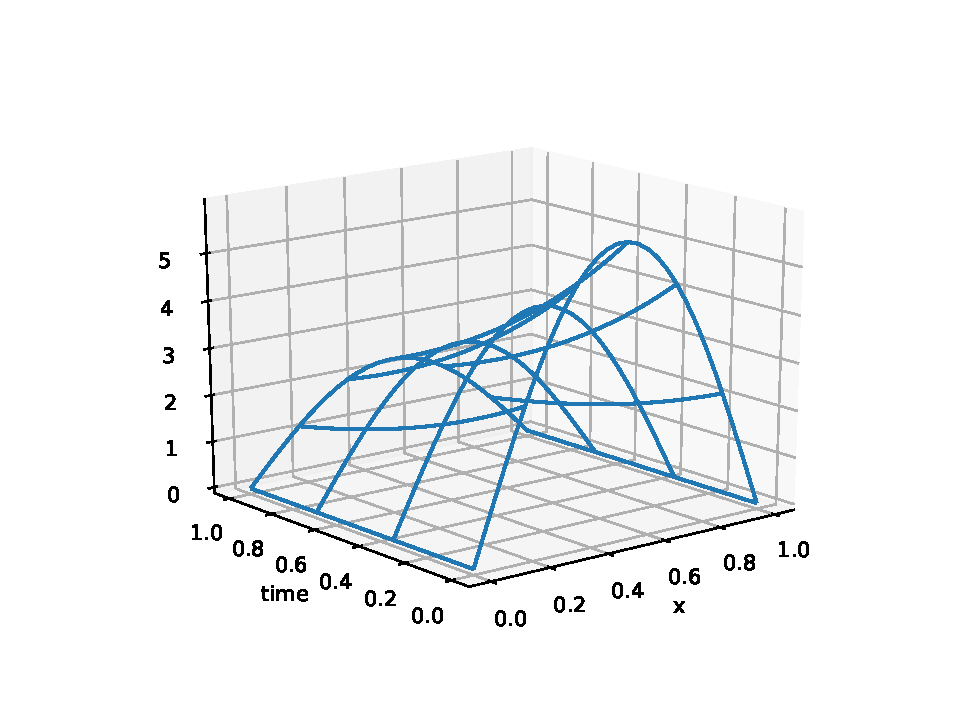
\includegraphics[width=0.5\textwidth]{Heat1.pdf}
   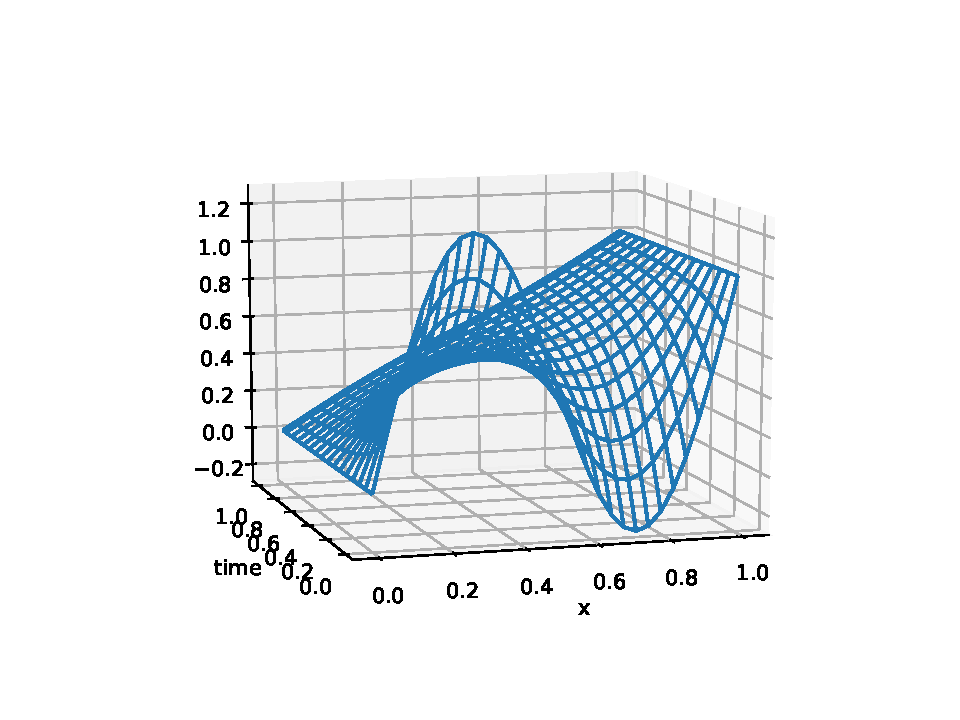
\includegraphics[width=0.5\textwidth]{Heat2.pdf}
   
 \caption{$f= 0$, $m=1$, $S = 1$, $k = \pi^-2$}
 \label{fig:Heat1}
\end{figure}



\clearpage

\section{The Finite Element Method} \label{sec:FEM}

This section is concerned with the discretisation of the Heat Equation by Finite Elements. Though not uncommon, the FEM is not necessarily widely known by the average postgraduate mathematician. As such we will provide a fairly detailed description of the method and full derivation of the scheme. A very nice introduction to the subject if more detail is needed is \cite{larson2013finite}.

The underlying practical steps to the method are:

\begin{enumerate}
\item Finding a variational form of the equation we are looking to solve. This will allow us to look for a solution which satisfies the equation in some weak sense. This step requires the introduction of the function spaces in which we can study our  equation and look for its solution. We will see that these spaces are Sobolev spaces.

\item Creating the subdivision of our domain $\Omega$.

\item Taking the variational form, which we have at first defined in an infinite dimensional function space $V$, and approximating it on a finite dimensional sub-space $V_{h}$. In our case the subspace will be piecewise polynomial functions defined on our subdivision.

\item Projecting the boundary conditions onto the finite dimensional space.
\end{enumerate}

\subsection{A subsection} \label{subsec:theory}

Subsections may be used. Use a clear structure in your report.

We denote the set of real numbers by
$\mathbb{R}$, the set of integers by $\ZZ$ and the set of complex
numbers by $\mathbb{C}$. Our analysis is based on the equation
$e^{\pi i} = -1$ and the relation
\begin{equation}
  \frac{2}{4} = \frac{1}{2}   \label{eq:myeq1}
\end{equation} % no empty line after this
which we verify in the appendix \ref{app:calculations}.
Useful consequences are
\begin{align}
  \frac{4}{8} &= \frac{1}{2} \\
  \frac{4}{12} + \frac{1}{\Gamma(s)}\int_0^{\infty} \frac{t^{s-1}}{e^t-1} dt
     &= \frac{1}{3} +\sum_{n=1}^{\infty} \frac{1}{n^s}\\
  \frac{2}{10} &= \frac{1}{5} 
\end{align}
For any $0\neq a\in \ZZ$, the equality
\begin{equation*} % * for no numbering
 \frac{2 a}{4 a} = \frac{1}{2}
\end{equation*}
follows from equation \eqref{eq:myeq1}.

\subsection{Another subsection} \label{subsec:application}

\subsubsection{A subsubsection} \label{subsubsec:red}

Sometimes subsubsections may be appropriate.

\subsubsection{Another subsubsection} \label{subsubsec:green}

This could contain a table of interesting numbers
\begin{center}
  \begin{tabular}{r|cccccc}
    $n$   & 1 & 2 & 3 & 4 & 5 & 6 \\ \hline
    $F_n$ & 1 & 1 & 2 & 3 & 5 & 8 \\
    $B_n$ & $\tfrac{1}{2}$ & $\tfrac{1}{6}$ & 0 & $-\tfrac{1}{30}$ & 0 &  $\tfrac{1}{42}$ \\
    $p_n$ & 2 & 3& 5& 7 & 11 & 13 \\
  \end{tabular}
\end{center}

\newpage


\section{A simple implementation} \label{sec:simpleFEM}




\newpage

\section{Error Analysis in the Finite Element Method} \label{sec:Errors}

\newpage

\section{Design of Adaptive Algorithms} \label{sec:Adaptive}

\newpage

\section{Some Numerical Examples} \label{sec:Adaptive}

\newpage

\section{Object oriented design patterns} \label{sec:my2}

Graphics can be included. Figure \ref{fig:bsd} shows an example.
Learn about floats and pictures in the \LaTeX\ wikibook to place
the figures at the right place in the end.
%
\begin{figure}[h]
 \begin{center}
 \end{center}
 \caption{Oh look, something happens here !}
 \label{fig:bsd}
\end{figure}

\newpage

\section{Conclusions} \label{sec:conclusions}

Further help on \LaTeX\ can be found easily on the internet. The \LaTeX\
wikibook\footnote{\tt http://en.wikibooks.org/wiki/LaTeX} contains a lot.
For instance you would find there how to type theorems and proofs nicely.
Or how to include source code written in some programming language like
matlab. There are long lists available with all sorts of common
mathematical symbols like $\xi$, $\nabla$, $\infty$, $\log$, $\iff$, etc.

\newpage

\appendix

\section{Raw data} \label{app:rawdata}

Material that needs to be included but would distract from the main
line of presentation can be put in appendices.
Examples of such material are raw
data, computing codes and details of calculations.


\section{Calculations for section \ref{sec:my1}} \label{app:calculations}

In this appendix we verify equation \eqref{eq:myeq1}.

\newpage

	\bibliography{References}
	\bibliographystyle{plain}

\end{document}
